\documentclass{report}
\usepackage{a4}
\usepackage[latin1]{inputenc}
%\usepackage[dvips]{graphicx}
\usepackage[pdftex]{graphicx}
\usepackage{verbatim}
\usepackage[total={6in, 9in}, top=1in,left=1.1in]{geometry} 
\usepackage{moreverb}
\usepackage{psfrag}
\usepackage{amsmath}
\usepackage[small]{caption}
\usepackage{amssymb}
\usepackage{fancyhdr}
\usepackage{shadow}            
\usepackage{setspace}
\usepackage{listings}
\usepackage{subfig}
\usepackage{upquote} %To make straigh quotes work in pdf

\setlength{\headheight}{12.5pt}
\newcommand{\undertilde}[1]{\underset{\widetilde{}}{#1}}
\newcommand{\HRule}{\rule{\linewidth}{0.5mm}}

\pagestyle{fancy}


\begin{document}

 \begin{titlepage}
  \begin{center}
 
 
	

	

        \HRule \\[0.4cm]
        Tutorial:\\[0.2cm]
	{ \huge \bfseries Connected Bodies in Proteus using the Chrono TSDA Class}\\[0.4cm]
	\HRule \\[1cm]

        \begin{minipage}{0.35\textwidth}
        Developed for proteus 1.7.5 and chrono 5.0 \newline \newline \newline \newline \newline \newline \newline \\
	\end{minipage}\\[1cm]

	

	\includegraphics[width=15cm]{TSDA_title.png}
	
	\vfill


	{\large \today}
	 
	\end{center}

 \end{titlepage}


\chapter*{Learning outcomes}

\noindent The reader will learn:\\[0.4cm]

\noindent{\bf How to use it:}
\begin{itemize}
\item how to use the ChLinkTSDA class to connect bodies in proteus
\item how to use proteus logging functions to record spring forces, velocities, and lengths
\item how to use some python scripts for post processing the information from these logs
\item basic post-processing of the simulation results in paraview
\end{itemize}
{\bf The theory of it:}
\begin{itemize}
\item the theory behind the ChLinkTSDA class
\end{itemize}


\chapter*{Prerequisites}

The reader is expected to have/know the following:
\begin{itemize}
\item Proteus 1.7.5+ compiled with chrono 5.0 installed in the proteus stack
\item any version of Paraview installed
\item the proteus tutorial folder downloaded on your PC (or access to git, so that you can git clone the folder from github) 
\item updated chrono logging definitions in the proteus/mbd/CouplingFSI.pyx file
\item How to run basic proteus simulations
\item How to setup simple floating body simulations in proteus
\end{itemize}

\tableofcontents


\chapter{Tutorial ChLinkTSDA}

\section{Introduction}

This tutorial describes how to pre-process, run and post-process a case involving compressible reacting flow with Lagrangian evaporating particles in a three-dimensional domain. It also describes how to copy the solver, copy an evaporation model and how to add a second material to the discrete particles. 
\newline \newline
The geometry consists of a block filled with air, with a 0.01x0.01 meter base and a length of 0.1 meter (figure \ref{geo1}). An injector is centrally placed on the top boundary where n-Heptane ($C_7H_{16}$) is injected. When the discrete droplets enter the domain they evaporate and combustion takes place in the gas phase. There are several gas phase reaction schemes supplied with the case  ranging from a reaction scheme with 5 species and one reaction up to a reaction scheme involving $\sim$300 reactions and 56 species.    
\begin{figure}[h]
  \centering
  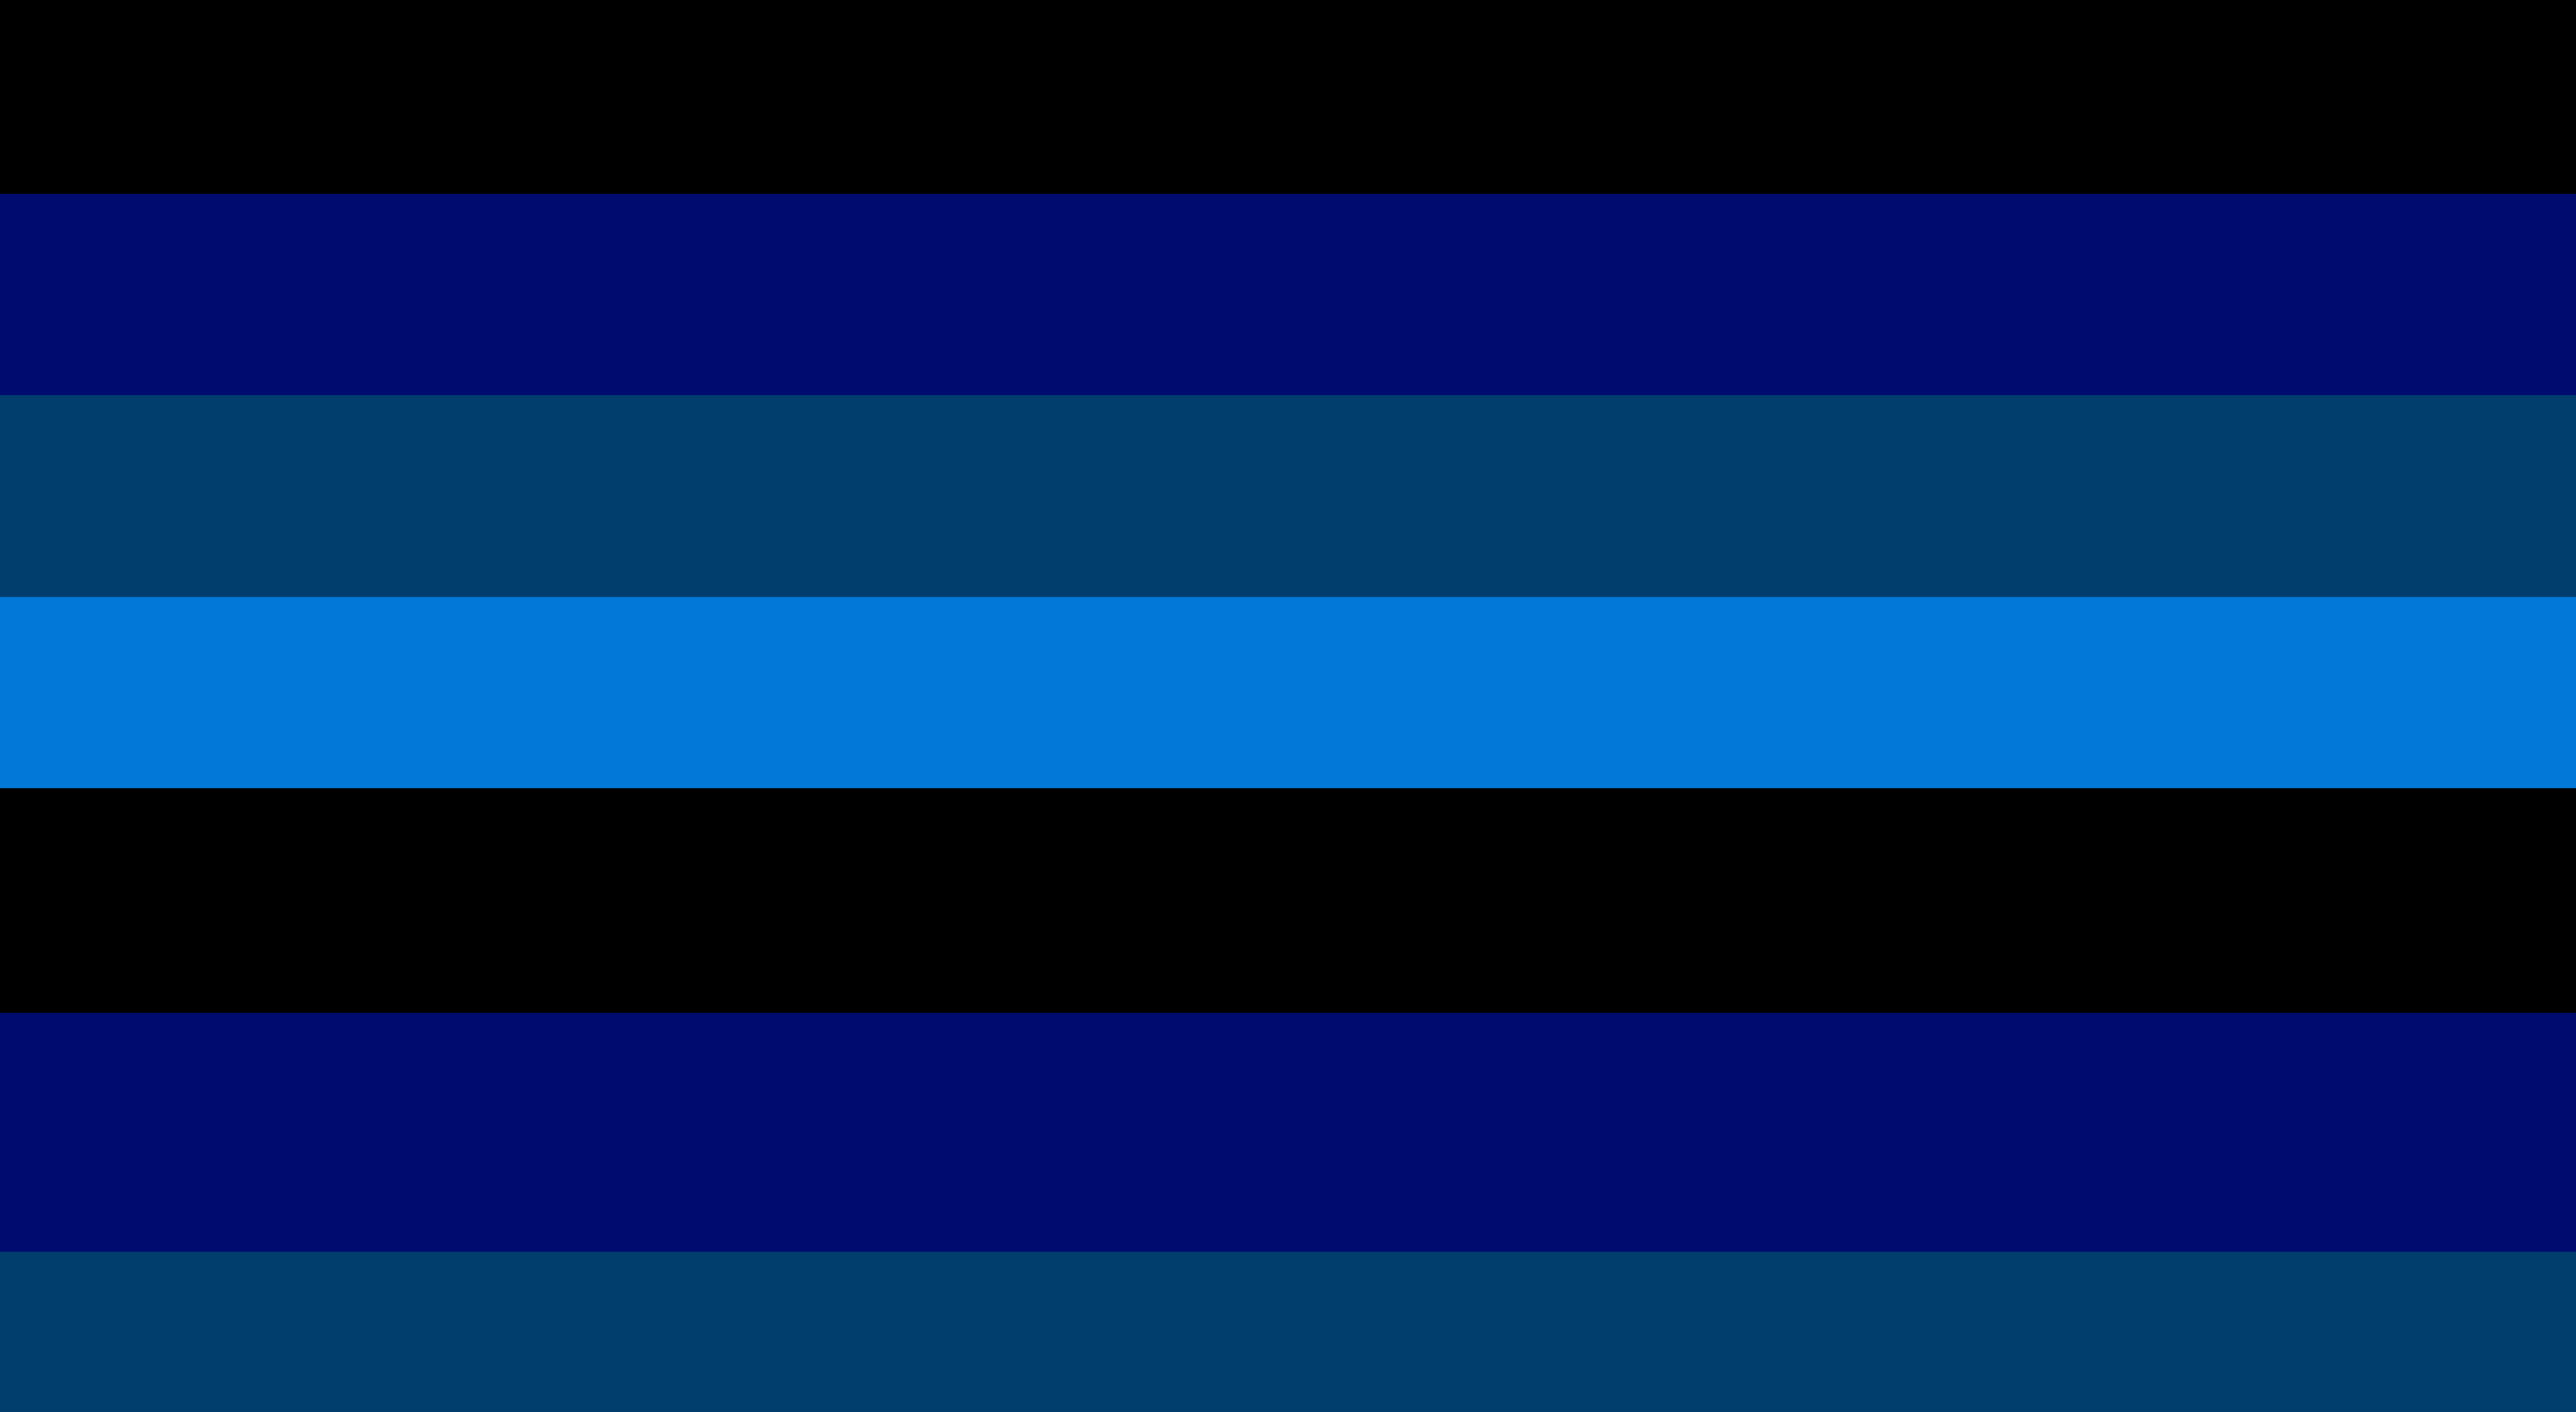
\includegraphics[width=4cm]{geo1.png}
  \setcaptionwidth{14cm}
  \caption{Geometry of the dieseFoam tutorial case.}
  \label{geo1}
\end{figure}
\newpage
\section{Pre-processing}

\end{document}
